\documentclass[12pt, titlepage]{article}

\usepackage{fullpage}
\usepackage[round]{natbib}
\usepackage{multirow}
\usepackage{booktabs}
\usepackage{tabularx}
\usepackage{graphicx}
\usepackage{float}
\usepackage{hyperref}
\usepackage{longtable}
\usepackage{ulem}
\hypersetup{
    colorlinks,
    citecolor=blue,
    filecolor=black,
    linkcolor=red,
    urlcolor=blue
}

\input{../../Comments}
\input{../../Common}

\newcounter{acnum}
\newcommand{\actheacnum}{AC\theacnum}
\newcommand{\acref}[1]{AC\ref{#1}}

\newcounter{ucnum}
\newcommand{\uctheucnum}{UC\theucnum}
\newcommand{\uref}[1]{UC\ref{#1}}

\newcounter{mnum}
\newcommand{\mthemnum}{M\themnum}
\newcommand{\mref}[1]{M\ref{#1}}

\begin{document}

\title{Module Guide for \progname{}} 
\author{\authname}
\date{\today}

\maketitle

\pagenumbering{roman}

\section{Revision History}

\begin{tabularx}{\textwidth}{p{3cm}p{2cm}X}
\toprule {\bf Date} & {\bf Version} & {\bf Notes}\\
\midrule
Jan 9, 2025 & 1.1 & Initial Document\\

\bottomrule
\end{tabularx}

\newpage

\section{Reference Material}

This section records information for easy reference.

\subsection{Abbreviations and Acronyms}

\renewcommand{\arraystretch}{1.2}
\begin{tabular}{l l} 
  \toprule		
  \textbf{symbol} & \textbf{description}\\
  \midrule 
  AC & Anticipated Change\\
  DAG & Directed Acyclic Graph \\
  M & Module \\
  MG & Module Guide \\
  OS & Operating System \\
  R & Requirement\\
  SC & Scientific Computing \\
  SRS & Software Requirements Specification\\
  \progname & Explanation of program name\\
  UC & Unlikely Change \\
  JWT & JSON Web Tokens \\
  MFA & Multi-Factor Authentication \\
  \bottomrule
\end{tabular}\\

\newpage

\tableofcontents

\listoftables

\listoffigures

\newpage

\pagenumbering{arabic}

\section{Introduction}

Decomposing a system into modules is a commonly accepted approach to developing
software.  A module is a work assignment for a programmer or programming
team~\citep{ParnasEtAl1984}.  We advocate a decomposition
based on the principle of information hiding~\citep{Parnas1972a}.  This
principle supports design for change, because the ``secrets'' that each module
hides represent likely future changes.  Design for change is valuable in SC,
where modifications are frequent, especially during initial development as the
solution space is explored.  

Our design follows the rules layed out by \citet{ParnasEtAl1984}, as follows:
\begin{itemize}
\item System details that are likely to change independently should be the
  secrets of separate modules.
\item Each data structure is implemented in only one module.
\item Any other program that requires information stored in a module's data
  structures must obtain it by calling access programs belonging to that module.
\end{itemize}

After completing the first stage of the design, the Software Requirements
Specification (SRS), the Module Guide (MG) is developed~\citep{ParnasEtAl1984}. The MG
specifies the modular structure of the system and is intended to allow both
designers and maintainers to easily identify the parts of the software.  The
potential readers of this document are as follows:

\begin{itemize}
\item New project members: This document can be a guide for a new project member
  to easily understand the overall structure and quickly find the
  relevant modules they are searching for.
\item Maintainers: The hierarchical structure of the module guide improves the
  maintainers' understanding when they need to make changes to the system. It is
  important for a maintainer to update the relevant sections of the document
  after changes have been made.
\item Designers: Once the module guide has been written, it can be used to
  check for consistency, feasibility, and flexibility. Designers can verify the
  system in various ways, such as consistency among modules, feasibility of the
  decomposition, and flexibility of the design.
\end{itemize}

The rest of the document is organized as follows. Section
\ref{SecChange} lists the anticipated and unlikely changes of the software
requirements. Section \ref{SecMH} summarizes the module decomposition that
was constructed according to the likely changes. Section \ref{SecConnection}
specifies the connections between the software requirements and the
modules. Section \ref{SecMD} gives a detailed description of the
modules. Section \ref{SecTM} includes two traceability matrices. One checks
the completeness of the design against the requirements provided in the SRS. The
other shows the relation between anticipated changes and the modules. Section
\ref{SecUse} describes the use relation between modules.

\section{Anticipated and Unlikely Changes} \label{SecChange}

This section lists possible changes to the system. According to the likeliness
of the change, the possible changes are classified into two
categories. Anticipated changes are listed in Section \ref{SecAchange}, and
unlikely changes are listed in Section \ref{SecUchange}.

\subsection{Anticipated Changes} \label{SecAchange}

Anticipated changes are the source of the information that is to be hidden
inside the modules. Ideally, changing one of the anticipated changes will only
require changing the one module that hides the associated decision. The approach
adapted here is called design for change.

\begin{description}
\item[\refstepcounter{acnum} \actheacnum \label{acLogin}:] The system should support different authentication methods, such as password-based, biometric login etc.
\item[\refstepcounter{acnum} \actheacnum \label{acTransSpeed}:] The transcription module needs to be optimized to enhance the transcription speed from audio data to written text in real-time. 
\item[\refstepcounter{acnum} \actheacnum \label{acPredModules}:] The diagnosis prediction and medicine prediction modules should be updated with the latest medical knowledge based on the new medical research.
\item[\refstepcounter{acnum} \actheacnum \label{acRealTime}:] The system shall enable real-time streaming of audio input to written text to ensure immediate transcription without delays.   
\end{description}

\subsection{Unlikely Changes} \label{SecUchange}

The module design should be as general as possible. However, a general system is
more complex. Sometimes this complexity is not necessary. Fixing some design
decisions at the system architecture stage can simplify the software design. If
these decision should later need to be changed, then many parts of the design
will potentially need to be modified. Hence, it is not intended that these
decisions will be changed.

\begin{description}
\item[\refstepcounter{ucnum} \uctheucnum \label{ucSecure}:] The requirement to secure patient's profile ensures confidentiality will remain a constant priority in the system.
\item[\refstepcounter{ucnum} \uctheucnum \label{ucCompatible}:] The ability of the system to be compatible with the latest versions of different operating systems such as Windows, Linux and macOS will remain a constant requirement.
\item[\refstepcounter{ucnum} \uctheucnum \label{ucnoisefree}:] The requirement to exclude the background noise while using transcription module is unlikely to change for accurately classification of the medical data.
\item[\refstepcounter{ucnum} \uctheucnum \label{uceaseofuse}:] The system's ease of use is anticipated to remain a constant requirement to allow them to focus on patient's care instead of struggling with the technology. 
\end{description}

\section{Module Hierarchy} \label{SecMH}

This section provides an overview of the module design. Modules are summarized in a hierarchy decomposed by secrets in Table \ref{TblMH}. The modules listed below, which are leaves in the hierarchy tree, are the modules that will actually be implemented.

\begin{description}
  \item [\refstepcounter{mnum} \mthemnum \label{mAM}:] App Module
  \item [\refstepcounter{mnum} \mthemnum \label{mUAM}:] User Authentication Module
  \item [\refstepcounter{mnum} \mthemnum \label{mAPIM}:] API Module
  \item [\refstepcounter{mnum} \mthemnum \label{mAVM}:] Administrator View Module
  \item [\refstepcounter{mnum} \mthemnum \label{mCVM}:] Client View Module
  \item [\refstepcounter{mnum} \mthemnum \label{mRGM}:] Report Generating Module
  \item [\refstepcounter{mnum} \mthemnum \label{mTM}:] Transcription Module
  \item [\refstepcounter{mnum} \mthemnum \label{mCM}:] Classification Module
  \item [\refstepcounter{mnum} \mthemnum \label{mDPM}:] Diagnosis Prediction Module
  \item [\refstepcounter{mnum} \mthemnum \label{mMPM}:] Medicine Prediction Module
  \item [\refstepcounter{mnum} \mthemnum \label{mAMM}:] Administrator Account Management Module
  \item [\refstepcounter{mnum} \mthemnum \label{mPAM}:] Patient Account Management Module
  \item [\refstepcounter{mnum} \mthemnum \label{mDDM}:] Diagnosis Data Module
  \item [\refstepcounter{mnum} \mthemnum \label{mMDM}:] Medicine Data Module

\end{description}

\begin{table}[h!]
\centering
\begin{tabular}{p{0.3\textwidth} p{0.6\textwidth}}
\toprule
\textbf{Level 1} & \textbf{Level 2}\\
\midrule
{Hardware-Hiding Module} & None \\
\midrule
\multirow{7}{0.3\textwidth}{Behaviour-Hiding Module} & \mref{mUAM}\\
& \mref{mAPIM}\\
& \mref{mAVM}\\
& \mref{mCVM}\\
& \mref{mDDM}\\
& \mref{mMDM}\\
\midrule

\multirow{3}{0.3\textwidth}{Software Decision Module} & \mref{mAM}\\
& \mref{mRGM}\\
& \mref{mTM}\\
& \mref{mCM}\\
& \mref{mDPM}\\
& \mref{mMPM}\\
& \mref{mAMM}\\
& \mref{mPAM}\\
\bottomrule

\end{tabular}
\caption{Module Hierarchy}
\label{TblMH}
\end{table}

\section{Connection Between Requirements and Design} \label{SecConnection}

The design of the system is intended to satisfy the requirements developed in
the SRS. In this stage, the system is decomposed into modules. The connection
between requirements and modules is listed in Table~\ref{TblRT}.

% \wss{The intention of this section is to document decisions that are made
%   ``between'' the requirements and the design.  To satisfy some requirements,
%   design decisions need to be made.  Rather than make these decisions implicit,
%   they are explicitly recorded here.  For instance, if a program has security
%   requirements, a specific design decision may be made to satisfy those
%   requirements with a password.}

\section{Module Decomposition} \label{SecMD}

Modules are decomposed according to the principle of ``information hiding'' proposed by \citet{ParnasEtAl1984}. The \emph{Secrets} field in a module decomposition is a brief statement of the design decision hidden by the module. The \emph{Services} field specifies \emph{what} the module will do without documenting \emph{how} to do it. For each module, a suggestion for the implementing software is given under the \emph{Implemented By} title. If the entry is \emph{OS}, this means that the module is provided by the operating system or by standard programming language libraries.  \emph{\progname{}} means the module will be implemented by the \progname{} software.

Only the leaf modules in the hierarchy have to be implemented. If a dash (\emph{--}) is shown, this means that the module is not a leaf and will not have to be implemented.

\subsection{Hardware Hiding Modules (\mref{mHH})}

\begin{description}
\item[Secrets:]The data structure and algorithm used to implement the virtual hardware.
\item[Services:]Serves as a virtual hardware used by the rest of the system. This module provides the interface between the hardware and the software. So, the system can use it to display outputs or to accept inputs.
\item[Implemented By:] OS
\end{description}

\subsection{Behaviour-Hiding Module}

\begin{description}
\item[Secrets:]The contents of the required behaviours.
\item[Services:]Includes programs that provide externally visible behaviour of the system as specified in the software requirements specification (SRS) documents. This module serves as a communication layer between the hardware-hiding module and the software decision module. The programs in this module will need to change if there are changes in the SRS.
\item[Implemented By:] --
\end{description}

\subsubsection{User Authentication Module (\mref{mUAM})} 

\begin{description}
\item[Secrets:] The implementation details of the authentication mechanism, including secure storage and validation of user credentials, session management, and MFA logic.
\item[Services:] This module handles user authentication, including:
\begin{itemize}
    \item Validating user credentials during login.
    \item Generating and validating session tokens.
    \item Managing password recovery and reset processes.
    \item Enforcing MFA where applicable.
    \item Logging authentication attempts for security auditing.
\end{itemize}
\item[Implemented By:] Spring, JWT
\item[Type of Module:] Abstract Object
\end{description}

\subsubsection{API Module (\mref{mAPIM})}

\begin{description}
\item[Secrets:] The logic for generating and validating OAuth tokens, handling API request routing, and defining access control policies for secure data sharing.
\item[Services:] This module provides:
\begin{itemize}
    \item OAuth 2.0-based authentication and authorization for external API consumers.
    \item Secure token generation, validation, and renewal.
    \item Routing requests from external systems to the relevant internal modules.
    \item Access control enforcement to protect sensitive data and resources.
\end{itemize}
\item[Implemented By:] Spring, OAuth 2.0
\item[Type of Module:] Library
\end{description}

\subsubsection{Administrator View Module (\mref{mAVM})}

\begin{description}
\item[Secrets:]User interface customization based on the administrative tools and functionality required by healthcare networks.
\item[Services:]Provide healthcare network adminstrators with tools to onboard, update, and remove thier network on the system. Provide healthcare network adminstrators with tools to add healthcare professionals under a healthcare network to the system.
\item[Implemented By:]TypeScript, React
\item[Type of Module:]Abstract Object
\end{description}

\subsubsection{Client View Module (\mref{mCVM})}

\begin{description}
\item[Secrets:]User interface customization based on the tools and functionality required by healthcare professionals.
\item[Services:]Provides healthcare professionals with tools to login, create, update, and delete patient records, provide diagnostic suggestions, and medication suggestions.
\item[Implemented By:]TypeScript, React
\item[Type of Module:]Abstract Object
\end{description}

\subsubsection{Diagnosis Data Module (\mref{mDDM})}

\begin{description}
  \item[Secrets:]Database schema for indexing strategies, and data caching mechanisms for efficient storage and retrieval.
  \item[Services:]Manages secure storage, retrieval, and updates of data related to diagnosis records. The ultimate purpose for this is to provide training data for the ciagnosis prediction module.
  \item[Implemented By:]MongoDB, Spring
  \item[Type of Module:]Record
\end{description}

\subsubsection{Medicine Data Module (\mref{mMDM})}

\begin{description}
  \item[Secrets:]Database schema for indexing strategies, and data caching mechanisms for efficient storage and retrieval.
  \item[Services:]Manages secure storage, retrieval, and updates of data related to drug records. The ultimate purpose for this is to provide training data for the medicine prediction module.
  \item[Implemented By:]MongoDB, Spring
  \item[Type of Module:]Record
\end{description}


\subsection{Software Decision Module}

\begin{description}
\item[Secrets:] The design decision based on mathematical theorems, physical facts, or programming considerations. The secrets of this module are
  \emph{not} described in the SRS.
\item[Services:] Includes data structure and algorithms used in the system that do not provide direct interaction with the user. 
  % Changes in these modules are more likely to be motivated by a desire to
  % improve performance than by externally imposed changes.
\item[Implemented By:] --
\end{description}


\subsubsection{App Module (\mref{mAM})}

\begin{description}
\item[Secrets:] The algorithm used to control and coordinate the flow of data between different modules.
\item[Services:] Facilitates communication between different independent modules and manages the state of the application.
\item[Implemented By:] React
\item[Type of Module:] Abstract Object
\end{description}

\subsubsection{Report Generation Module (\mref{mRGM})}

\begin{description}
\item[Secrets:] The algorithm to generate accurate reports based on the transcribed data from the conversation.
\item[Services:] Extracts the important aspects of medical data and compiled into the report.
\item[Implemented By:] Python
\item[Type of Module:] Library
\end{description}

\subsubsection{Transcription Module (\mref{mTM})}

\begin{description}
\item[Secrets:] The algorithm used to convert audio data into written text.
\item[Services:] Accurately converts the audio data from the conversation into written text.   
\item[Implemented By:] Python
\item[Type of Module:] Library
\end{description}

\subsubsection{Classification Module (\mref{mCM})}

\begin{description}
\item[Secrets:] The algorithm used to classify the medical data after the transcription module.
\item[Services:] Accurately classifies the medical data received from the transcription module into relevant categories.
\item[Implemented By:] Python
\item[Type of Module:] Library
\end{description}

\subsubsection{Diagonsis Prediction Module (\mref{mDPM})}

\begin{description}
\item[Secrets:] The algorithms used to predict possible diagnoses.
\item[Services:] Predicts a set of applicable diagnoses for a patient based on patient characteristics, symptoms, and past medical history.
\item[Implemented By:] Python
\item[Type of Module:] Abstract Object
\end{description}

\subsubsection{Medicine Prediction Module (\mref{mMPM})}

\begin{description}
\item[Secrets:] The algorithms used to give possible medicines applicable.
\item[Services:] Predicts a set of applicable medicines for a patient based on patient characteristics, symptoms, and past medical history.
\item[Implemented By:] Python
\item[Type of Module:] Abstract object
\end{description}

\subsubsection{Administrator Account Management Module (\mref{mAMM})}

\begin{description}
\item[Secrets:]Database schema for indexing strategies, and data caching mechanisms for efficient storage and retrieval.
\item[Services:]Manages secure storage, retrieval, and updates of data related to healthcare networks and healthcare professionals.
\item[Implemented By:]MongoDB, Spring
\item[Type of Module:]Record
\end{description}

\subsubsection{Patient Account Management Module (\mref{mPAM})}

\begin{description}
\item[Secrets:]Database schema for indexing strategies, and data caching mechanisms for efficient storage and retrieval.
\item[Services:]Manages secure storage, retrieval, and updates of data related to patient records.
\item[Implemented By:]MongoDB, Spring
\item[Type of Module:]Record
\end{description}


\section{Traceability Matrix} \label{SecTM}

This section shows traceability matrices: between the modules and the requirements and between the modules and the anticipated changes.

% the table should use mref, the requirements should be named, use something
% like fref
\begin{table}[H]
\centering
\begin{tabular}{p{0.2\textwidth} p{0.6\textwidth}}
\toprule
\textbf{Req.} & \textbf{Modules}\\
\midrule
FR1 & \mref{mAM}, \mref{mAPIM}, \mref{mAVM}, \mref{mAMM}\\
FR2 & \mref{mAM}, \mref{mUAM}, \mref{mAPIM}, \mref{mAVM}, \mref{mAMM}\\
FR3 & \mref{mAM}, \mref{mUAM}, \mref{mAPIM}, \mref{mAVM}, \mref{mAMM}\\
FR4 & \mref{mAM}, \mref{mUAM}, \mref{mAPIM}, \mref{mAVM}, \mref{mAMM}\\
FR5 & \mref{mAM}, \mref{mUAM}, \mref{mAPIM}, \mref{mAVM}, \mref{mAMM}\\
FR6 & \mref{mAM}, \mref{mUAM}, \mref{mAPIM}, \mref{mAVM}, \mref{mAMM}\\
FR7 & \mref{mAM}, \mref{mUAM}, \mref{mAPIM}, \mref{mAMM}\\
FR8 & \mref{mAM}, \mref{mUAM}, \mref{mAPIM}, \mref{mCVM}, \mref{mPAM}\\
FR9 & \mref{mAM}, \mref{mUAM}, \mref{mAPIM}, \mref{mCVM}, \mref{mPAM}\\
FR10 & \mref{mAM}, \mref{mUAM}, \mref{mAPIM}, \mref{mCVM}, \mref{mPAM}\\
FR11 & \mref{mAM}, \mref{mUAM}, \mref{mAPIM}, \mref{mCVM}, \mref{mRGM}, \mref{mTM}, \mref{mCM}, \mref{mPAM}\\
FR12 & \mref{mAM},\mref{mUAM}, \mref{mAPIM}, \mref{mCVM}, \mref{mRGM}, \mref{mDPM}, \mref{mPAM}, \mref{mDDM}\\
FR13 & \mref{mAM}, \mref{mUAM}, \mref{mAPIM}, \mref{mCVM}, \mref{mRGM}, \mref{mMPM}, \mref{mPAM}, \mref{mMDM}\\
FR14 & \mref{mAM}, \mref{mUAM}, \mref{mAPIM}, \mref{mAVM}, \mref{mPAM}\\
\bottomrule
\end{tabular}
\caption{Trace Between Functional Requirements and Modules}
\label{TblRT}
\end{table}

\begin{table}[H]
\centering
\begin{tabular}{p{0.2\textwidth} p{0.6\textwidth}}
\toprule
\textbf{Req.} & \textbf{Modules}\\
\midrule
NFR1 & \mref{mAM}, \mref{mAVM}, \mref{mCVM}\\
NFR2 & \mref{mAM}, \mref{mAVM}, \mref{mCVM}\\
NFR3 & \mref{mAM}, \mref{mTM}\\
NFR4 & \mref{mAM}, \mref{mAMM}, \mref{mPAM}, \mref{mDDM}, \mref{mMDM}\\
NFR5 & All \\
NFR6 & \mref{mAM}, \mref{mUAM}, \mref{mPAM}\\
NFR7 & \mref{mAM}, \mref{mCVM}\\
NFR8 & All \\
NFR9 & All \\
\bottomrule
\end{tabular}
\caption{Trace Between Non-Functional Requirements and Modules}
\label{TblRT}
\end{table}


\begin{table}[H]
\centering
\begin{tabular}{p{0.2\textwidth} p{0.6\textwidth}}
\toprule
\textbf{Req.} & \textbf{Modules}\\
\midrule
AC1 & \mref{mAPIM}\\
AC2 & \mref{mAM}, \mref{mUAM}, \mref{mAPIM}, \mref{mAVM}, \mref{mAMM}\\
IR1 & \mref{mUAM}, \mref{mAPIM}, \mref{mAVM}, \mref{mAMM}\\
IR2 & All \\
IR3 & \mref{mDPM}, \mref{mMPM}\\
IR4 & \mref{mAMM}, \mref{mPAM}\\
IR5 & \mref{mDPM}, \mref{mMPM}\\
IR6 & \mref{mRGM}, \mref{mCM}\\
IR7 & \mref{mRGM}, \mref{mTM}\\
\bottomrule
\end{tabular}
\caption{Trace Between Safety and Security Requirements and Modules}
\label{TblRT}
\end{table}

\begin{table}[H]
\centering
\begin{tabular}{p{0.2\textwidth} p{0.6\textwidth}}
\toprule
\textbf{AC} & \textbf{Modules}\\
\midrule
\acref{acLogin} & \mref{mAM}, \mref{mUAM}\\
\acref{acTransSpeed} & \mref{mTM}\\
\acref{acPredModules} & \mref{mDPM}, \mref{mMPM}\\
\acref{acRealTime} & \mref{mAM}, \mref{mAPIM}, \mref{mCVM}, \mref{mTM}, \mref{mcM}\\
\bottomrule
\end{tabular}
\caption{Trace Between Anticipated Changes and Modules}
\label{TblACT}
\end{table}

\section{Use Hierarchy Between Modules} \label{SecUse}

In this section, the uses hierarchy between modules is
provided. \citet{Parnas1978} said of two programs A and B that A {\em uses} B if
correct execution of B may be necessary for A to complete the task described in
its specification. That is, A {\em uses} B if there exist situations in which
the correct functioning of A depends upon the availability of a correct
implementation of B.  Figure \ref{FigUH} illustrates the use relation between
the modules. It can be seen that the graph is a directed acyclic graph
(DAG). Each level of the hierarchy offers a testable and usable subset of the
system, and modules in the higher level of the hierarchy are essentially simpler
because they use modules from the lower levels.

\wss{The uses relation is not a data flow diagram.  In the code there will often
be an import statement in module A when it directly uses module B.  Module B
provides the services that module A needs.  The code for module A needs to be
able to see these services (hence the import statement).  Since the uses
relation is transitive, there is a use relation without an import, but the
arrows in the diagram typically correspond to the presence of import statement.}

\wss{If module A uses module B, the arrow is directed from A to B.}

\begin{figure}[H]
\centering
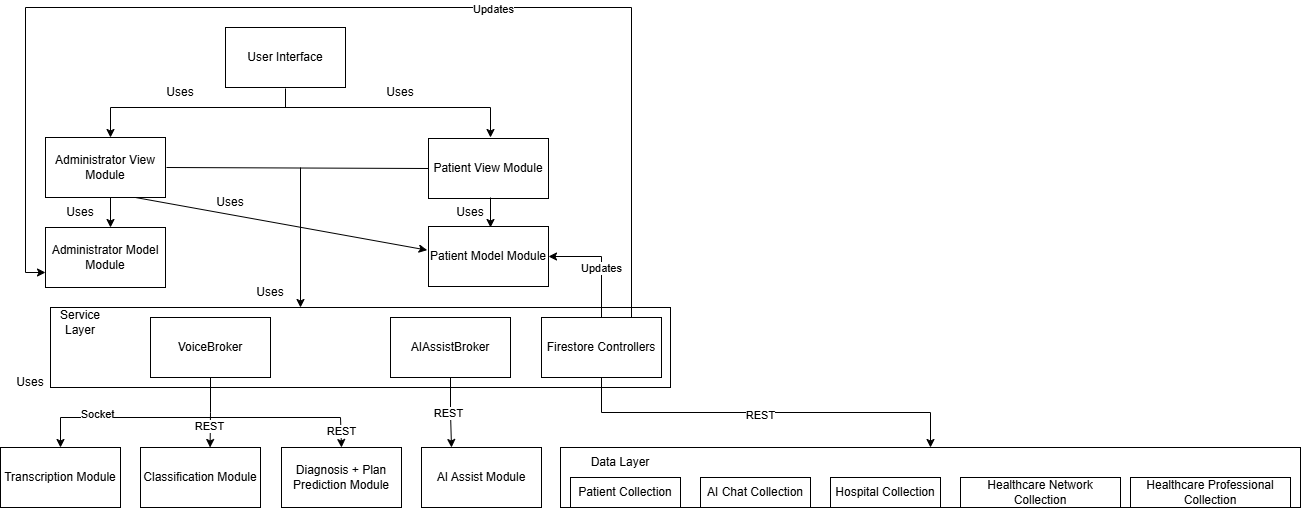
\includegraphics[width=0.7\textwidth]{user-hierarchy.png}
\caption{Use hierarchy among modules}
\label{FigUH}
\end{figure}

%\section*{References}

\section{User Interfaces}

\wss{Design of user interface for software and hardware.  Attach an appendix if
needed. Drawings, Sketches, Figma}

\section{Design of Communication Protocols}

Due to the broker architectures connecting with various services, the communication protocols differ slightly. For most of the communication as they will be simply `POST` or `GET`. Examples of this communication being used would be fetching patient data from the database, classifying the transcription, or employee retrieval, etc... HTTP communication will be used in \textbf{all} but one use case.

The one use case where HTTP communication will not be used is for the transcription service. For this service we will be using web socket communication as this will provide streaming capabilities for real time transcription. The frontend will act as the client who will send audio chunks to the backend to be transcribed. This will facilitate bidirectional communcation as well.


\section{Timeline}



\bibliographystyle {plainnat}
\bibliography{../../../refs/References}

\newpage{}

\end{document}